%%This is a very basic article template.
%%There is just one section and two subsections.
\documentclass[times,10pt,twocolumn,letterpaper]{article}
\usepackage{color}
\usepackage{ncvpripg}
\usepackage{times}
\usepackage[pdftex]{graphicx}	
\usepackage[cmex10]{amsmath}
\usepackage{url}
\usepackage{hyperref} 

\title{Stagnant Water Detection in Urban Area Using quadcopter}
\author{}
\def\iccvPaperID{238}
\begin{document}
\maketitle

\begin{abstract}
Recently, in urban areas there has been a sharp increase in dengue and malaria.
One of the major reason for this is suspected to be the amount of stagnant
water around residencies. There are many areas around urban residential places
such as terraces of high rise buildings, and shades above windows
(popularly known as `chhajja') that are hard to reach and hence to inspect. We
used quadcopter to inspect such areas and detect whether there is stagnant
water. We have proposed a method which combines Support Vector Machine (SVM)
based classifer with optical flow based technique to reliably detect the
stagnant water puddle in the captured video. Qualitative comparison shows
superiority of our method over method available in literature.

\end{abstract}

\section{Introduction}
{\color{red} [MGP] Need to cut short the introduction}

Dengue~\cite{WHO15Dengue} and Malaria~\cite{WHO15Malaria} are among the deadly
diseases common in at least 100 countries all over the world with exception of
Europe continent. In India itself there are around one million Malaria
cases~\cite{NVBDP_Malaria} and fourty thousand cases of
dengue~\cite{NVBDP_Dengue} in year 2014. The disease is transmitted by the
biting of mosquitoes and if not appropriately treated, people may have
recurrences of the disease months later~\cite{Cecilia14}. These mosquitoes
flourish during rainy seasons but can breed in water-filled flower pots,
plastic bags, and cans year-round. Stagnant water is major site for breeding of
these mosquitoes.

The risk of disease can be reduced by preventing mosquito bites by using
mosquito nets and insect repellents. Also, we may take mosquito-control
measures such as spraying insecticides, fogging etc. China has reportedly
used sterile mosquitoes~\cite{china} to fight dengue fever.  But, such measures
may prove dangerous to environment as well as eco-system. Plus, even though major
measures are in exercise, we have not succeeded in eradicating these diseases. One of
the major reasons behind this may be the continuous existence of water-puddles
around urban residential places.

Some areas such as high rise buildings' terraces, construction sites, area
near water storage (having possible leakages/overflows) etc. does not attract
attention easily. So, we need an effective mechanism to keep an ``eye'' on such
areas to detect presence of stagnant water. 

Microsoft \cite{Microsoft15} have started ``Project Premonition'' which aims to
use drones to catch mosquitoes for detection of pathogens in them before these
pathogens make people sick. But for sending drones to catch mosquitoes we first
need to find out possible mosquito breeding areas such as water puddles. We
propose a method in which we manuevere a quadcopter to record video of the
whole place, and later process that video to identify the frames which contain
water puddle, which will in turn aid in the process of identifying particular
areas for further action.

\begin{figure}[h!]
\centering
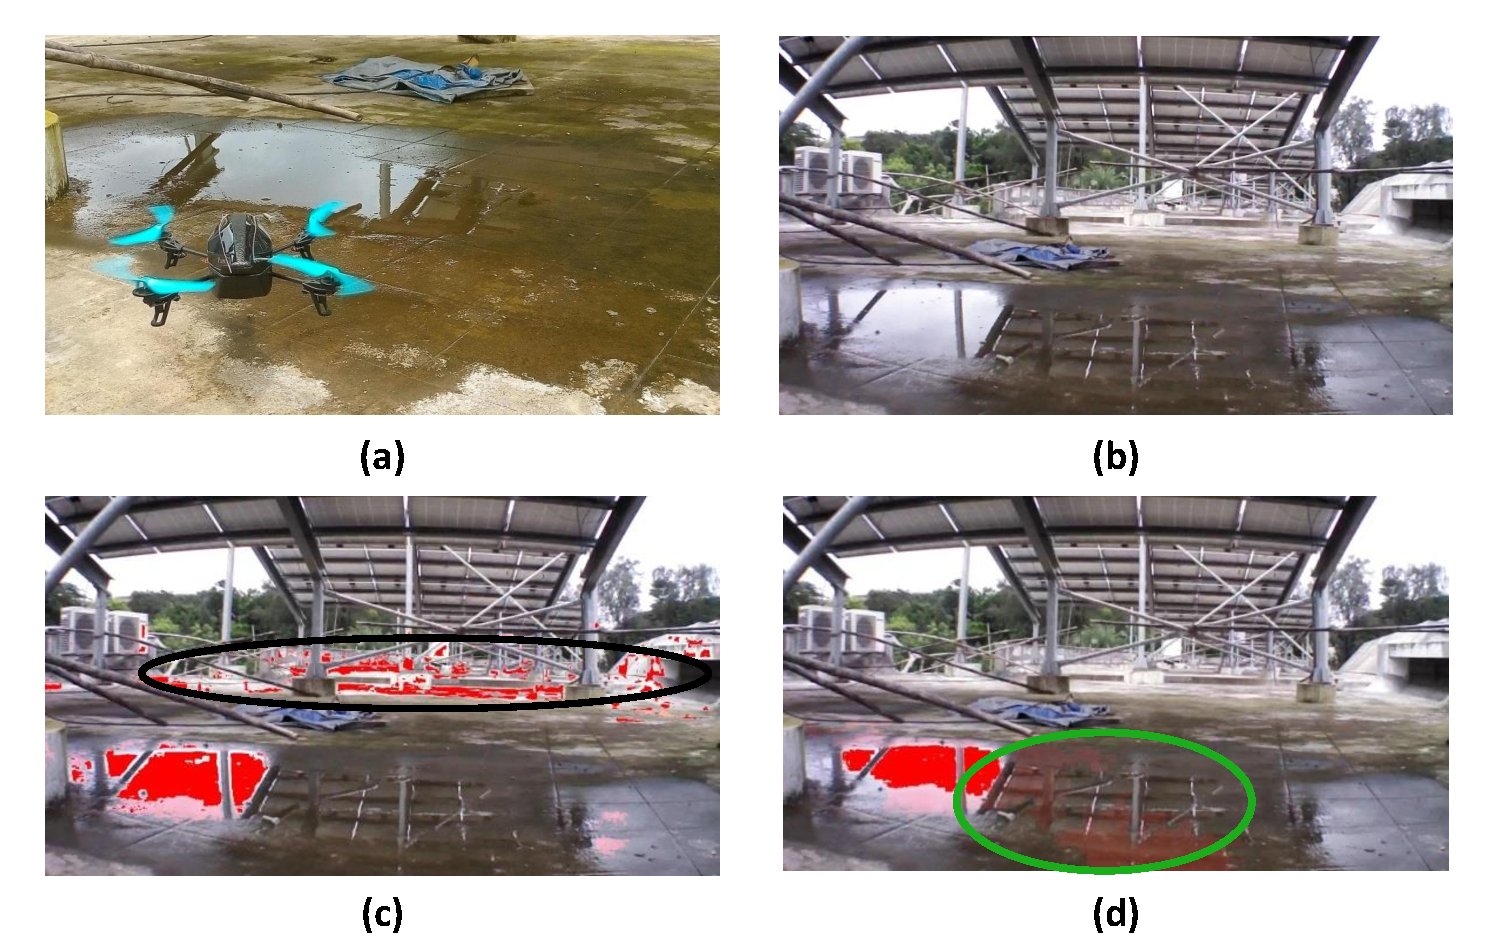
\includegraphics[width=\linewidth]{images/teaser.pdf}
\caption{(a) Quadcopter hovering over stagnant water amassed at building
backyard. (b) Scene captured by quadcopter (c) Our algorithm is able to detect
puddle region in the scene (shown in red).}
\end{figure}

\section{Related Work}

Rankin et al.~\cite{rankin04} have detected the presence of water from color,
texture, and the detection of reflections in stereo range data. They have used a
rule base for fusing water cues which was developed by evaluating detection
results from an extensive archive of data collection imagery containing water.
In another work, Rankin et al.~\cite{rankin11} have implemented a water detector
based on sky reflections that geometrically locates the pixel in the sky that
is reflecting on a candidate water pixel on the ground and predicts if the
ground pixel is water based on color similarity and local terrain features. 

Santana et al.~\cite{santana12}'s method for detection of water relies on the
chaotic nature of water’s dynamic texture to exploit a measure of entropy over the
trajectories obtained from optical flow trackers over several frames.

Zhang et al.~\cite{zhang10} have introduced a descriptor which is tolerant
to the flip transformation and even non-rigid distortions, such as ripple
effects (in additon to invariant to scales, rotations and affine
transformations) to detect water reflections.

\section{Methodology}
In this section we will see the three approaches; SVM classifier with HSV
histogram based feature, Optical flow based technique, and finally combination
of these two approaches to detect stagnant water robustly.

\subsection{SVM classifier}

\begin{figure}[h!]
\centering
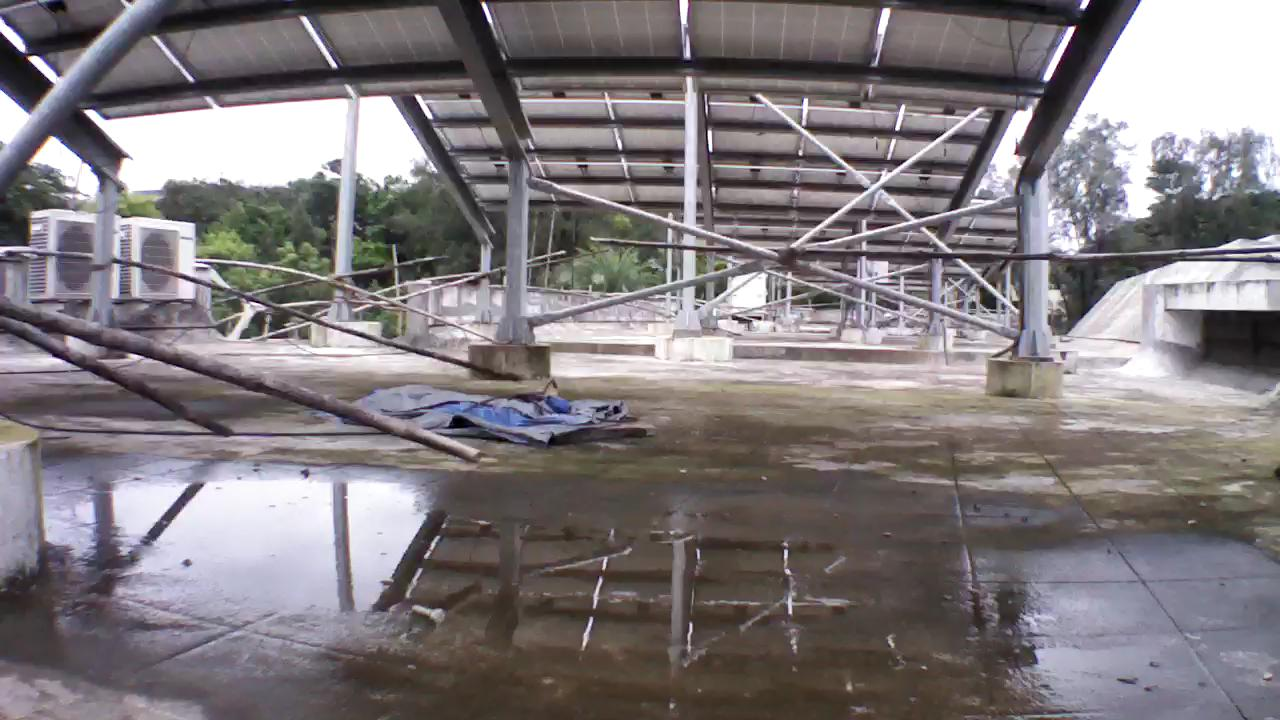
\includegraphics[width=0.22\linewidth]{images/IMG_PAIR_27_1.jpg}
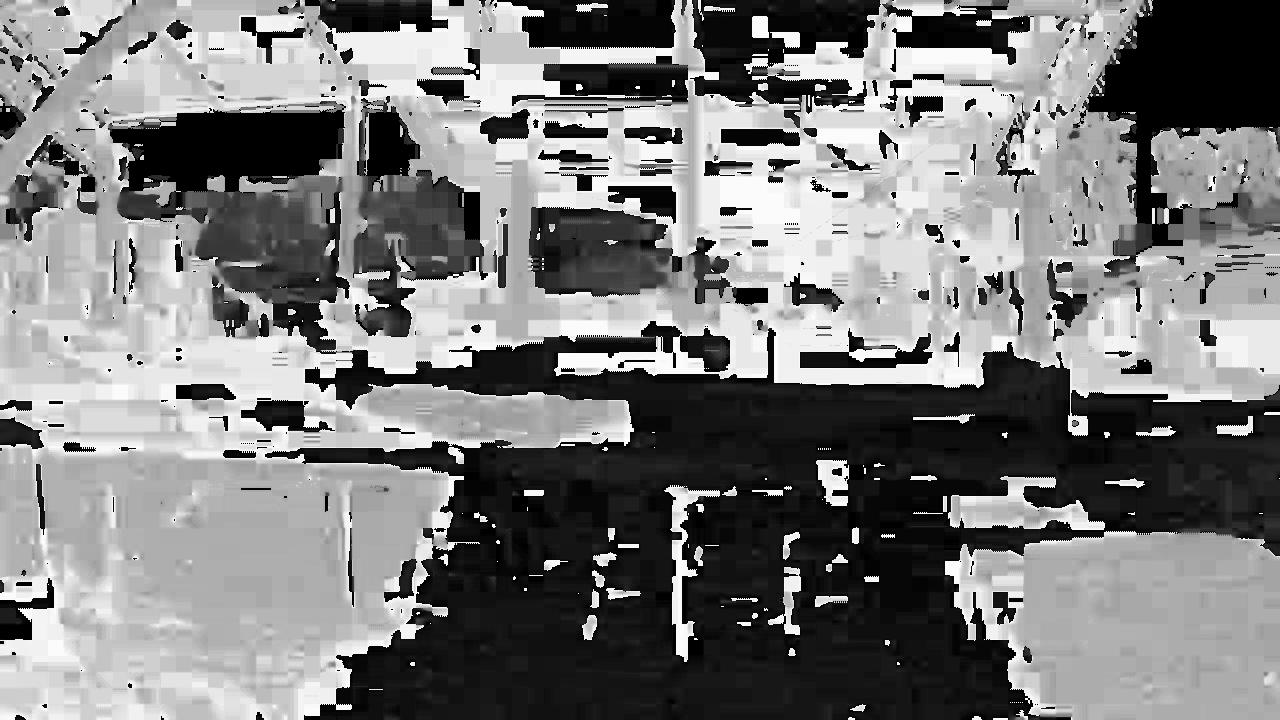
\includegraphics[width=0.22\linewidth]{images/IMG_PAIR_27_1_H.jpg}
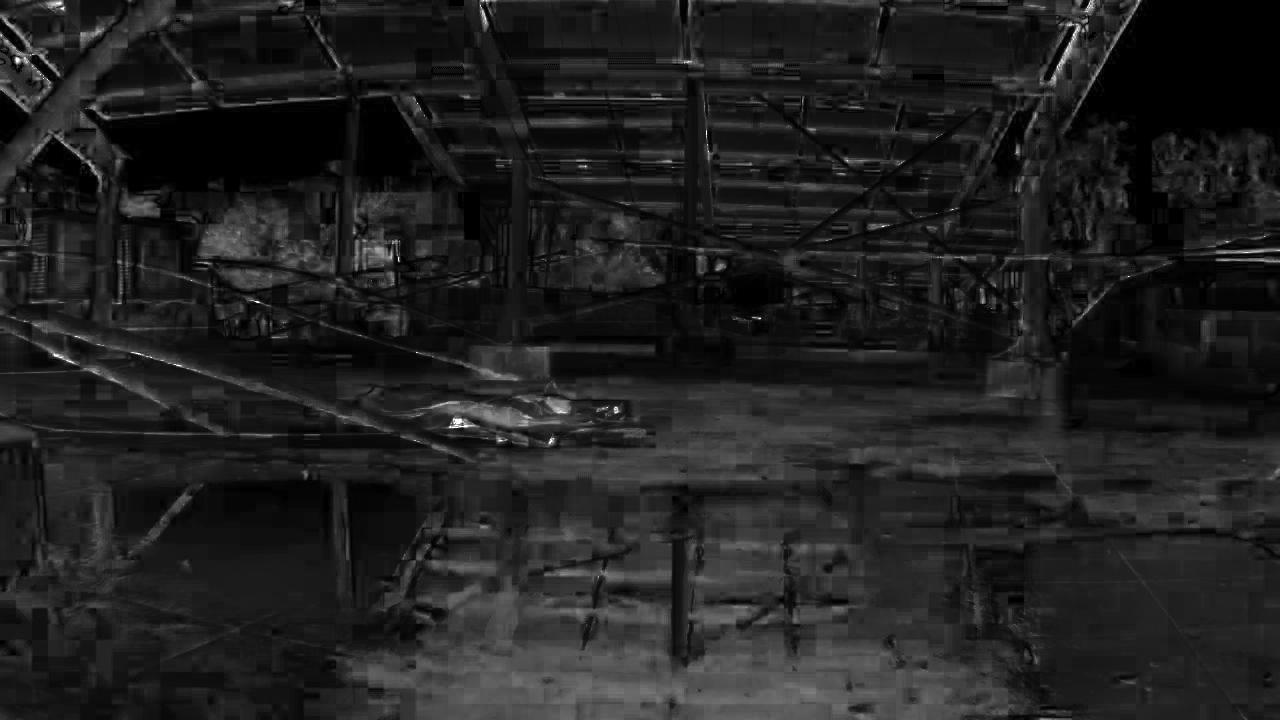
\includegraphics[width=0.22\linewidth]{images/IMG_PAIR_27_1_S.jpg}
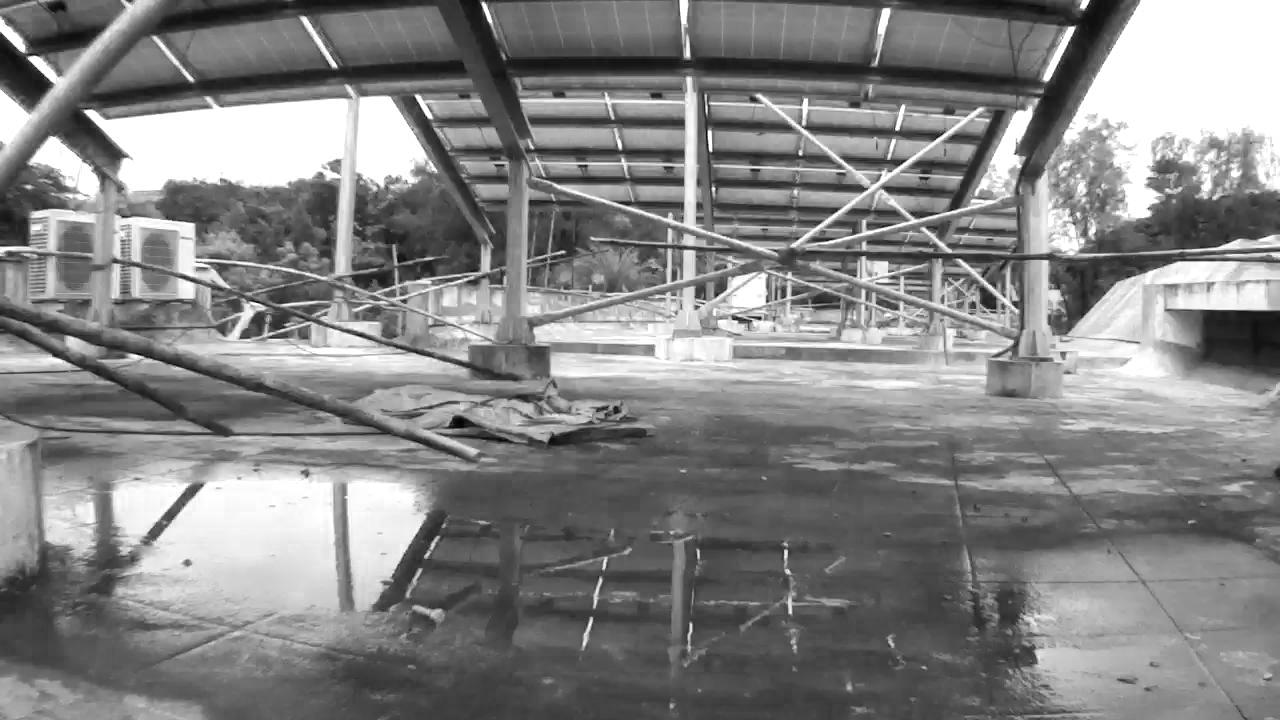
\includegraphics[width=0.22\linewidth]{images/IMG_PAIR_27_1_V.jpg}
\caption{Sample image and their Hue (H), Saturation (S) and Value (V) components
respectively. It can be seen that puddle area has very less Saturation. Also,
reflective parts of puddle has high intensity.}
\label{fig:HSV}
\end{figure}

Under ambient lighting conditions, puddle areas display high brightness and low
saturation~\cite{rankin04}. Hence, features that capture this information locally
could be used for puddle detection. Hence, considering a square image patch of
small side dimension, $n$, a novel feature is used that performs the following
steps:
\begin{enumerate}
\item Image is transformed from RGB color domain to HSV color space.
\item Histogram for each channel having k bins is constructed
\item The histogram values for three channels are concatenated to form a vector
of length $3k$.
\end{enumerate}
 
Here, to capture sufficient statistics as well as constrain the feature size,
number of bins, k = 64 is chosen, such that each bin contains 4 consecutive gray
levels. Also, the side of square patch is taken as $n = 50$ to capture local
characteristics.

The given feature is used to train a Support Vector Machine(SVM) using a
dataset of positively and negatively marked puddle patches. The
positively-labelled as well as negatively-labelled patches are manually marked
from a grid of size $m$ pixels overlaid on frames captured using quadcopter.
Since RBF kernels have been useful to efficiently detect
textures~\cite{Chapelle99}, it has been used for the given classifier. In our
experiments, values of $m = 16$ is used.

\subsubsection{Creation of training Data}
We have created a tool to select training data for the classifier. In this tool,
image will be shown in grid fashion with block size of $50  \times 50$. 
User will be enabled to draw contour over the desired region (puddle or
non-puddle). The blocks enclosed by the contour will be selected. Additionally
user may select additonally select blocks or deselect the selected blocks. The
proces is shown in Figure~\ref{fig:training}.

\begin{figure}[h!]
\centering
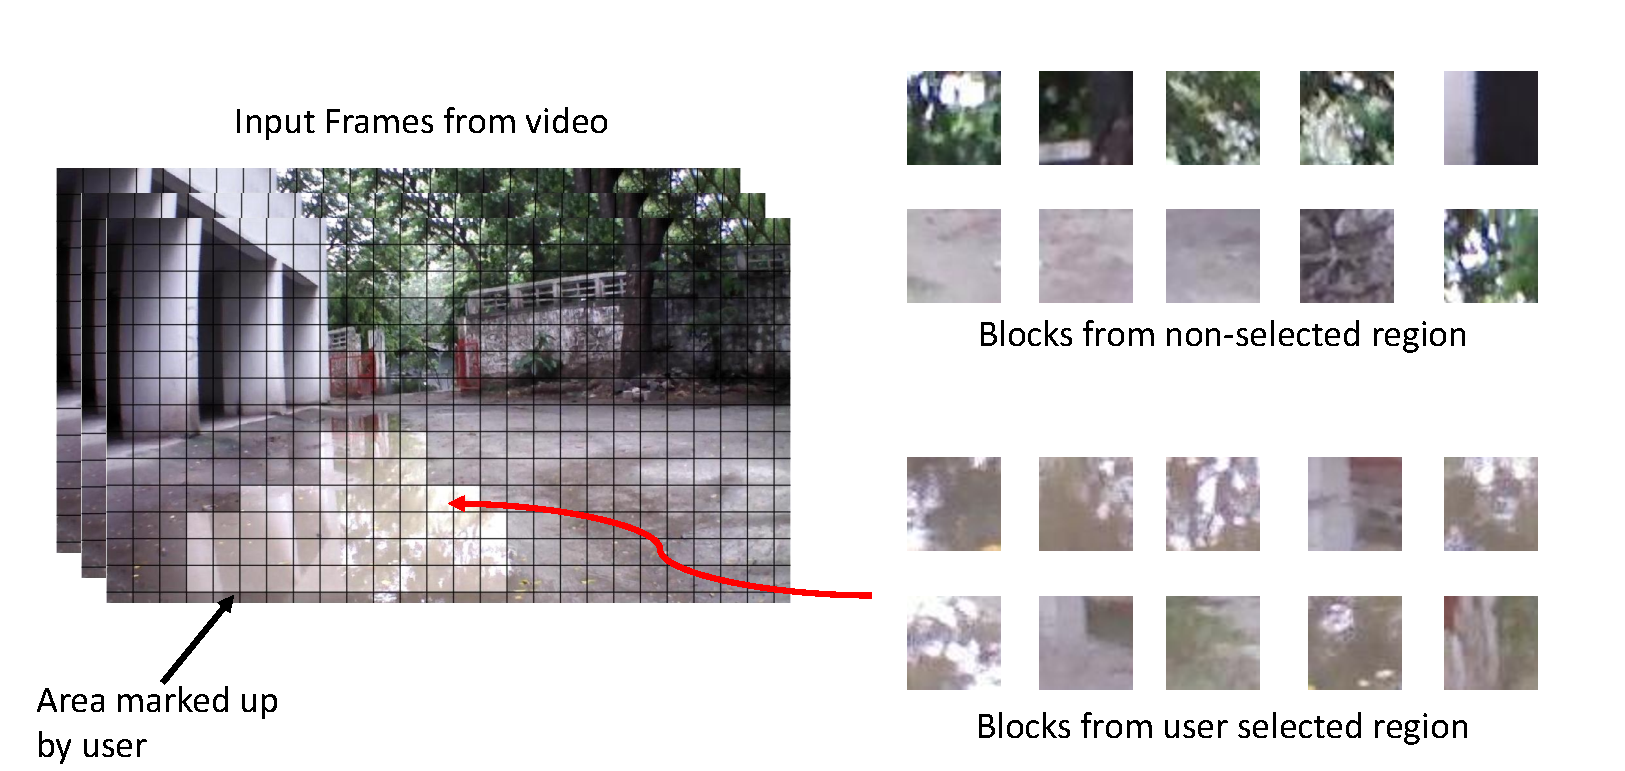
\includegraphics[width=\linewidth]{images/trainingData.pdf}
\caption{Process for creation of training data. User selects puddle area by
drawing a contour over input frame (using our tool). User can additionally
select/deselect blocks which he/she thinks are belonging to puddle/non-puddle
area. We use blocks covered by user drawn contour as `positive' training data.
Similarly, the `negative' training data may be selected.}
\label{fig:training}
\end{figure}

\textbf{Failure cases of SVM :- }
The svm detector is strong at detecting regions of sky reflected off a puddle.
In the HSV color space, these regions have low saturation (S) and high
brightness (V) values, and are picked up with high reliability by the HSV
histogram feature based SVM detector. However, other reflected regions such as
trees, buildings, etc. are usually classified as non-puddle regions as these
are labeled as such in the training images.

\subsection{Optical flow based technique}
Optical flow measures apparent motion of objects in a scene caused by relative
motion between camera and object. Hence, magnitude of optical flow will be high
for near objects while objects at large distance it will be low. Figure
\ref{fig:optical_flow} shows the magitude of optical flow calculated from two images
captured from quadcopter, consisting of water puddle region. 

\begin{figure}[h!]
\centering
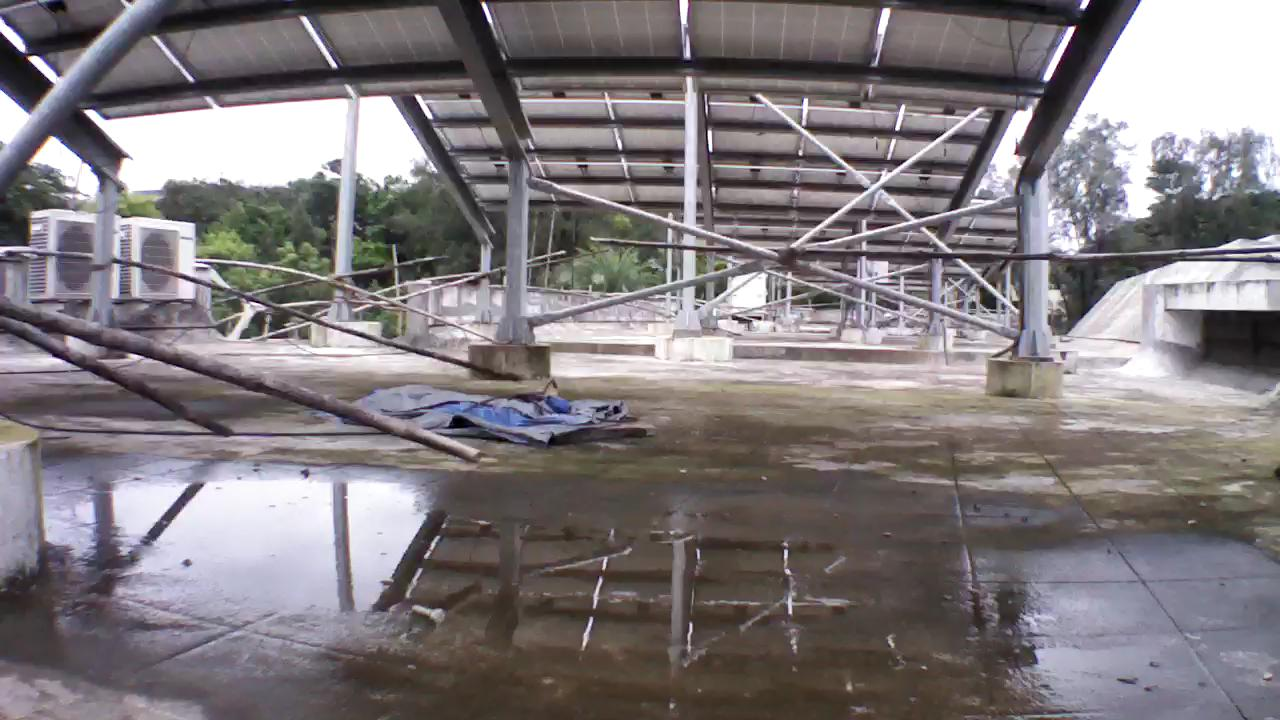
\includegraphics[width=0.3\linewidth]{images/IMG_PAIR_27_1.jpg}
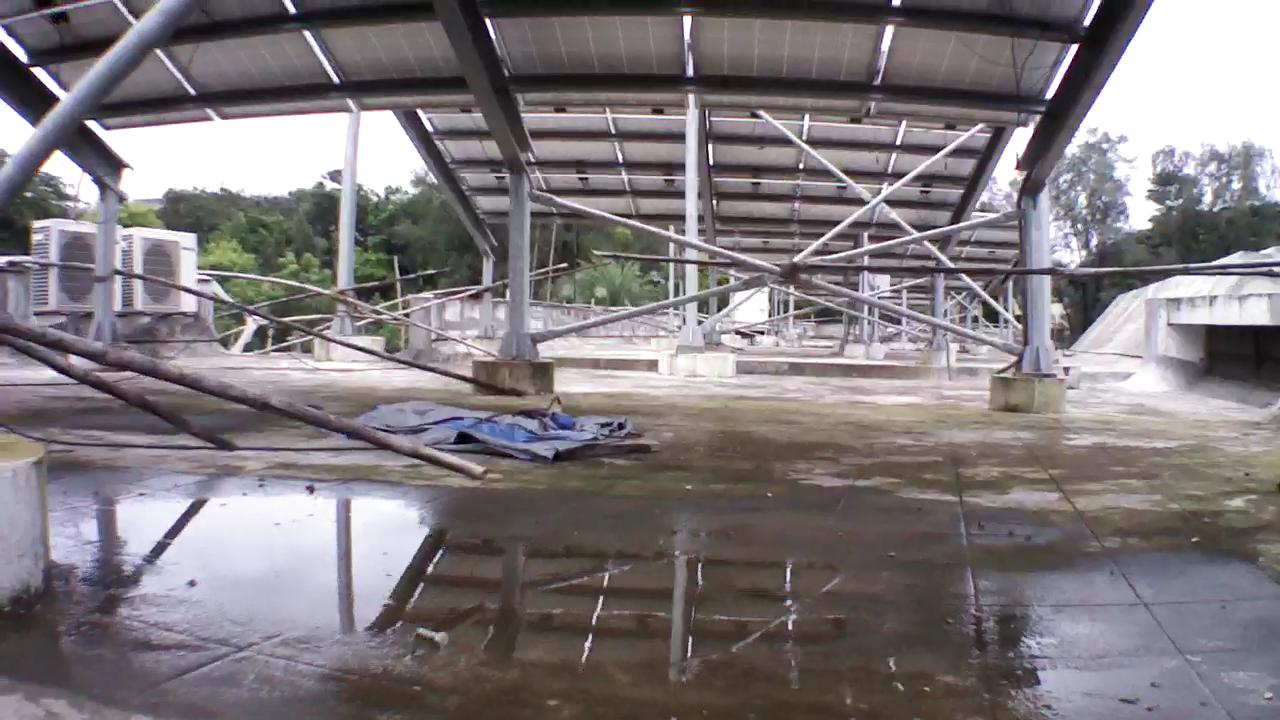
\includegraphics[width=0.3\linewidth]{images/IMG_PAIR_27_2.jpg}
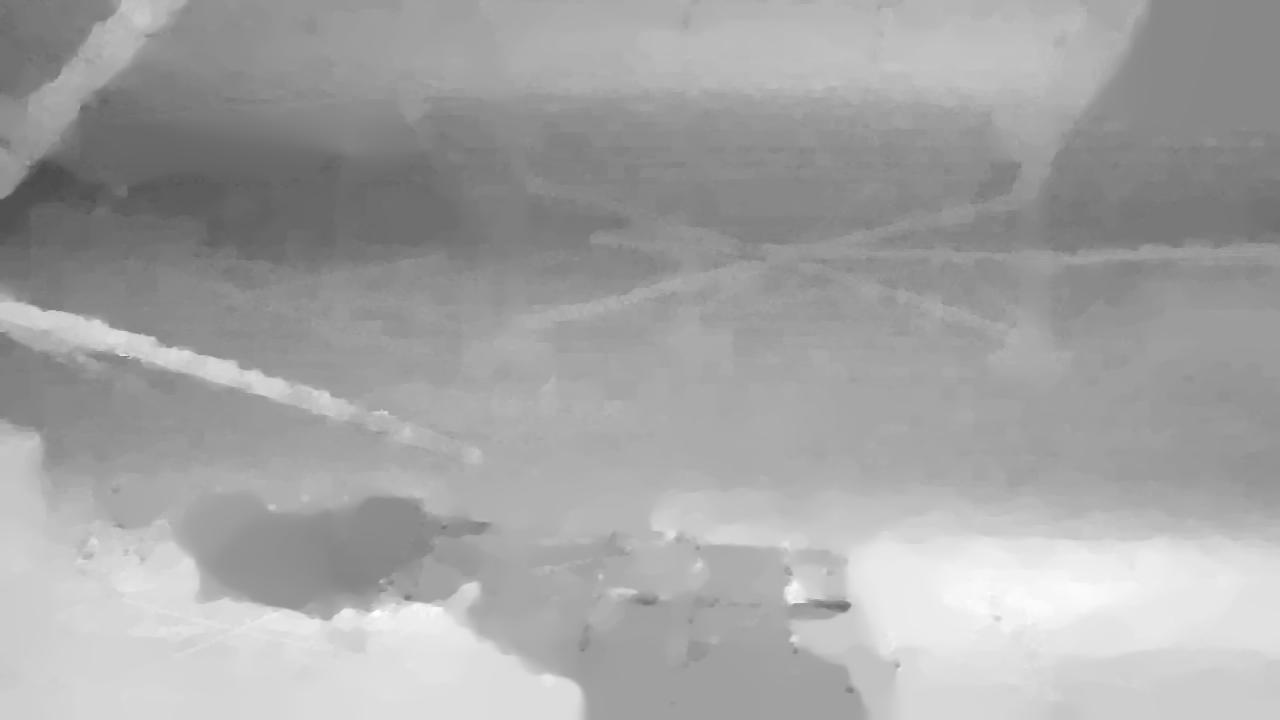
\includegraphics[width=0.3\linewidth]{images/IMG_PAIR_27_optical_flow.jpg}
\caption{Optical Flow. Left, middle: video frames taken from positions
which are $d$ units apart in 3D world. $ 0.01 \leq d \leq 0.1$. Right:
Magnitude of optical flow calculated from earlier images. Magnitude of optical
flow in the reflective parts of the puddle is low compared to that of its
suroundings.}
\label{fig:optical_flow}
\end{figure}

It can be seen that, the reflective part of the puddle have less optical flow
magnitude compared to its neighborhood. The reason behind this is, the
reflected objects being quite far from the actual puddle, the relative motion
will be less compared to its neighbourhood. So, we can use this property to
detect water puddle regions from the image.

We are using an algorithm  developed by Ce Liu~\cite{Liu11Thesis} which is based
on \cite{Brox04,Bruhn05} to find out optical flow. (The Matlab/C++ code for this
algorithm is given in \cite{Liu11}). \cite{Brox04} needs spatio-temporal
smoothness constraint. Temporal smoothness may be assured by taking adjacent (or
near djacent) frames from video. But, adhering to spatial smoothness constraint
is very difficult in case of UAV. 

Quadcopter provides us a way to enforce the spatial smoothness constraint on
the input images. We record Inertial Measurment Unit (IMU) data
transmitted by quadcopter, which in turn provides us the approximate position of
the quadcopter at given time. Later, we synchronize it with the video sequence
captured by quadcopter, to find out approximate position from which the given
frame is captured. Finally, we select frame pair which is nearest, among set of
temporally adjacent frames to find out the optical flow.

\textbf{Failure cases of optical flow}
Optical flow is essentially being used in a depth from parallax mode to exploit
the fact that still puddles behave like mirrors and scenery reflected by such
puddles is usually at a much greater depth than the immediate surroundings of
the puddle. Correspondingly, optical flow as a means of detecting puddles will
fail when the above assumption fails, such as when the reflected objects are
close by. Optical flow also generates false positives when the scene contains a
far off portion partially occluded by nearby objects.

\subsection{Combined approach}
\begin{figure}[h!]
\centering
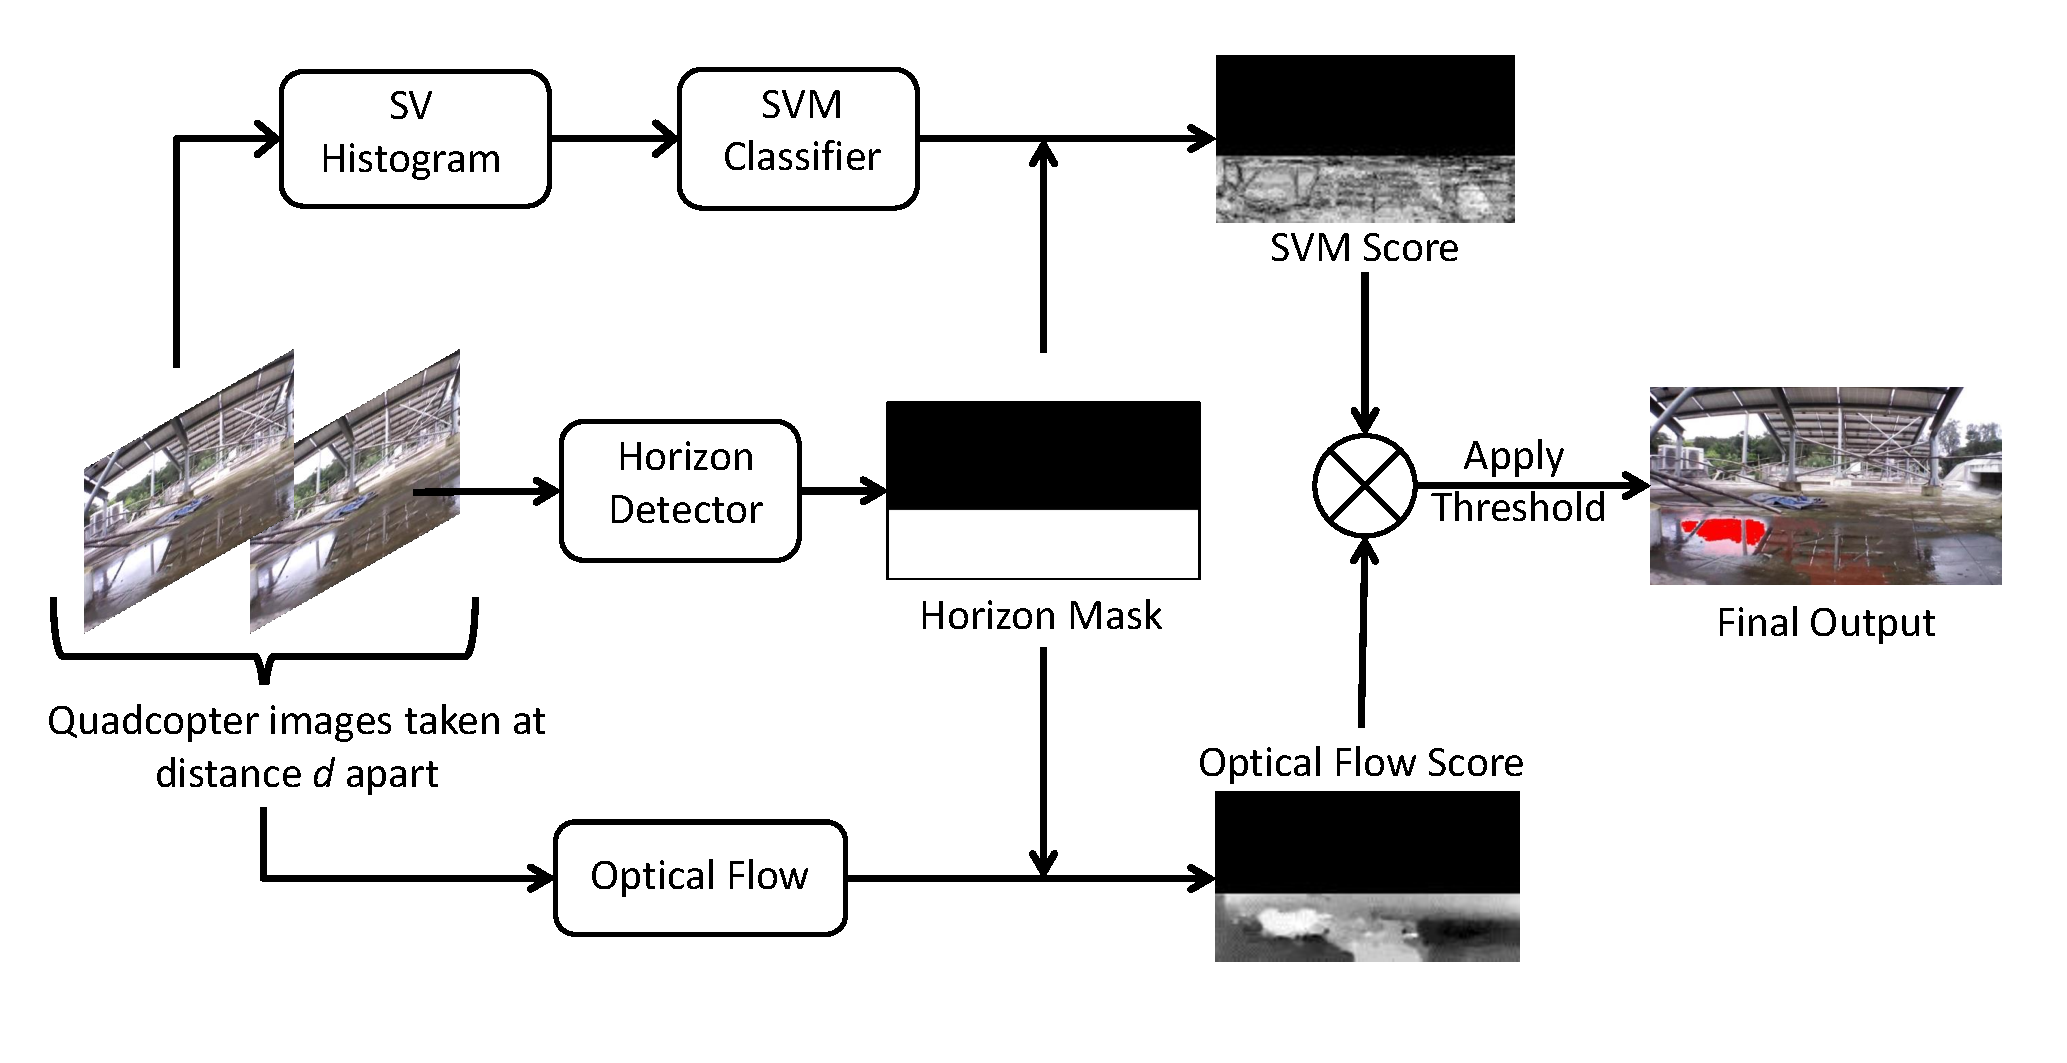
\includegraphics[width=\linewidth]{images/overall_workflow.pdf}
\caption{Overall workflow to detect stangant water.}
\label{fig:workflow}
\end{figure}

As illustrated in Figure \ref{fig:workflow}, first we select frames in
pairs from the captured video. Basically, the two frames which are
spatially as well temporally near are chosen as a pair.  Now, first frame will
be sent to SVM classifier to find the SVM score, while pair is used to find the
optical flow magnitude. Meanwhile we find out horizon from the first image to
filter in possible puddle areas. 

\textbf{Horizon Detection :- }
The change in depth for far-away scenes as well as their reflections on puddle,
in consecutive frames, are hard to distinguish. In previous work \cite{rankin11}
such issues are avoided by discarding a fixed-portion of image corresponding to
far-off regions, enforced by constrained input capture method. Due to
inapplicability of such constraints in comparatively agile input capture
conditions of quadcopter, features derived from urban environment are utilized
for finding plausible puddle regions. In urban setting, the high availability
of structures in surroundings, having distinctly flat surfaces and rectilinear
silhouettes, enables use of edge-detection based methods to bound planar
regions that can contain puddle. Applying hough transform with calibrated
parameters followed by length-based selection of lines detected, a upper
boundary for puddle region called `Horizon' is found. The Horizon is in turn
used to create a binary mask to be applied to local scores from other
techniques before normalization.

The SVM scores are obtained from classifier correspond to each patch of size, m
( m = 16 as mentioned in section), while for computational efficiency, optical
flow is performed on frames downsampled to half of the original dimensions.
But, to obtain a combined estimate based on both techniques, scores for a
common patch size are necessary. Hence, the optical flow scores are divided
into a grid of size $m/2$ pixels, each sub-patch of which are averaged to
obtain the final optical flow score.

The combined score obtained from optical flow and SVM classifier provides a
probabilistic estimate of corresponding patch belonging a puddle. But, in order
to include contribution towards the estimate based on neighbourhood
information, a sequence of morphological operations are applied on the
combined score. From the resulting score, a mask denoting puddle region is
obtained by thresholding based on statistical parameters.

\section{Experiments and Results}
All our experiments have been completed with the inexpensive consumer
quadcopter called a Parrot's AR Drone 2.0. We have used the ROS based
ARDrone Autonomy Driver to communicate with the drone. For the purpose
of showing the efficacy of this paper, we also took a picture of the
scene from a distance with a 5 mega-pixel camera to better understand
the scene. Primarily we covered urban places such as terraces, constructions
sites, building backyards, pumping stations etc.

We have implemented our algorithm in Matlab R2014a. Experiments were performed
on a PC with Intel Core i7 processor(@3.4GHz) and 8GB RAM.  The source code
detect stagnant water regions in images from a video, as well as the data sets
used in this paper will be made publicly available.

\subsection{Comparison with prior technique}
Comparison of proposed method's output and \cite{rankin04} on representative
images on some of the datasets is shown in Figure \ref{fig:comparison}.

\begin{figure}
\centering
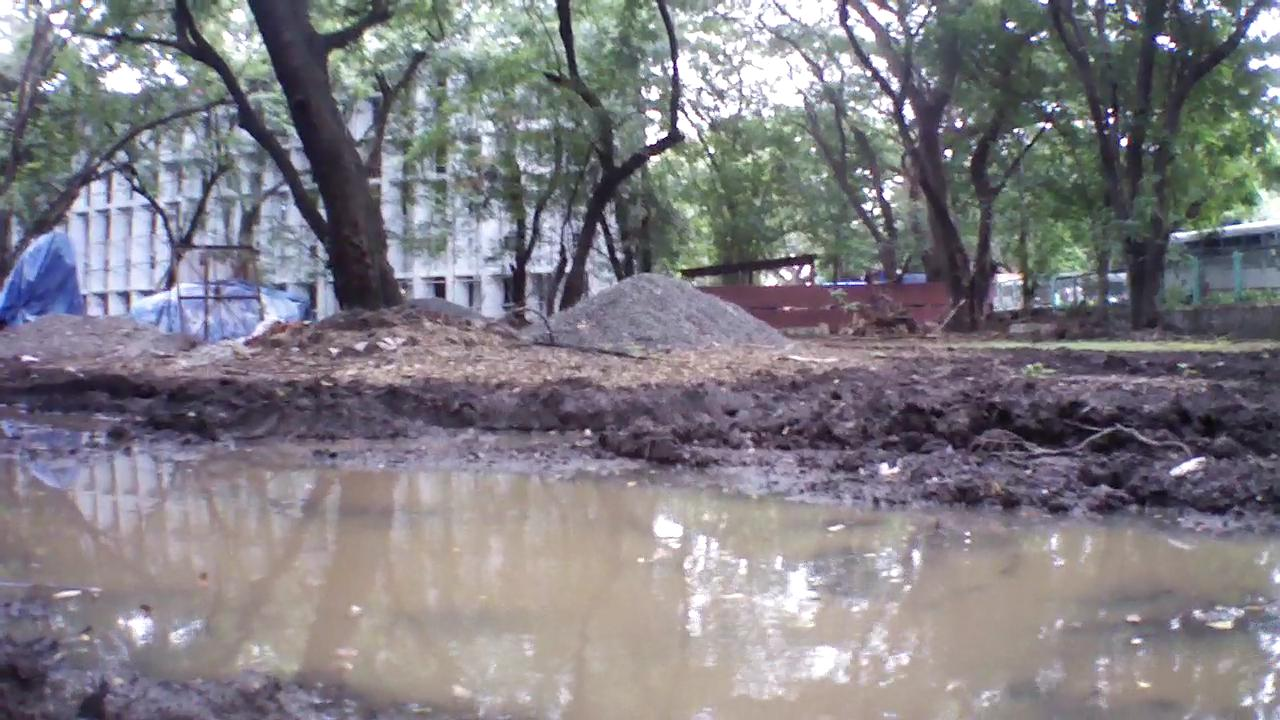
\includegraphics[width=0.31\linewidth]{images/results/dataset_63full/IMG_PAIR_102_1.jpg}
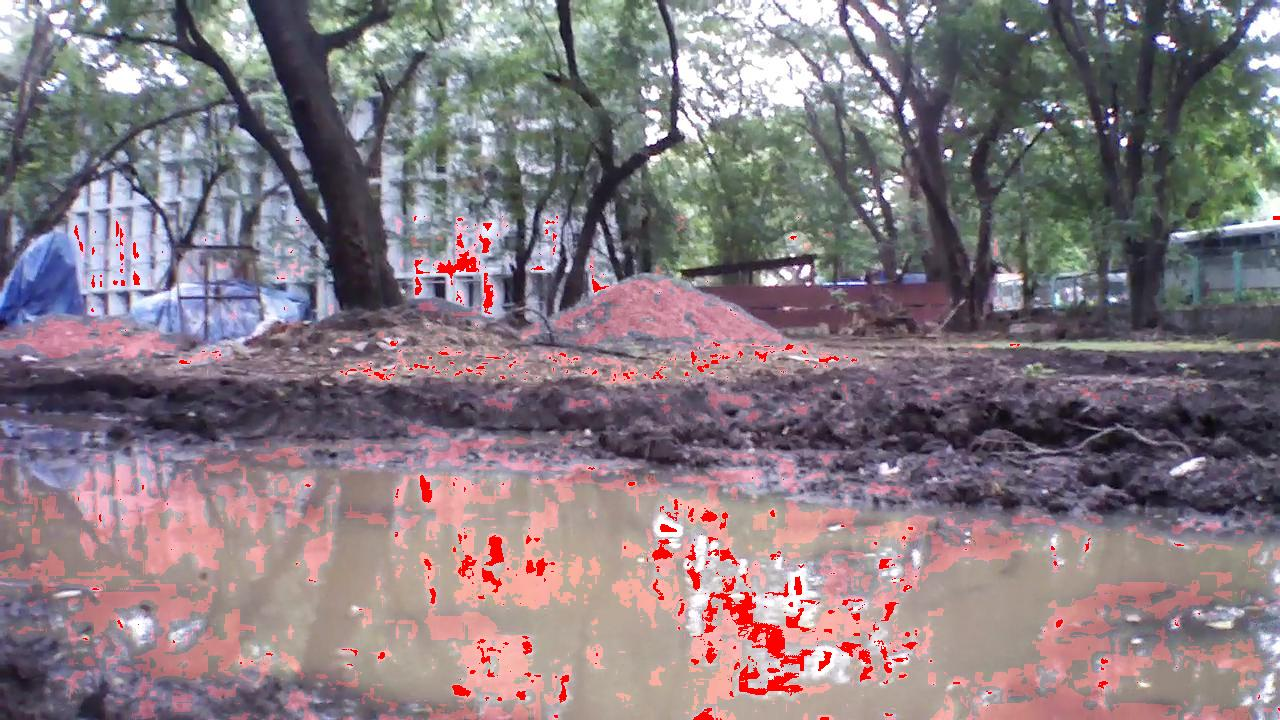
\includegraphics[width=0.31\linewidth]{images/results/dataset_63full/output_102_jpl2.jpg}
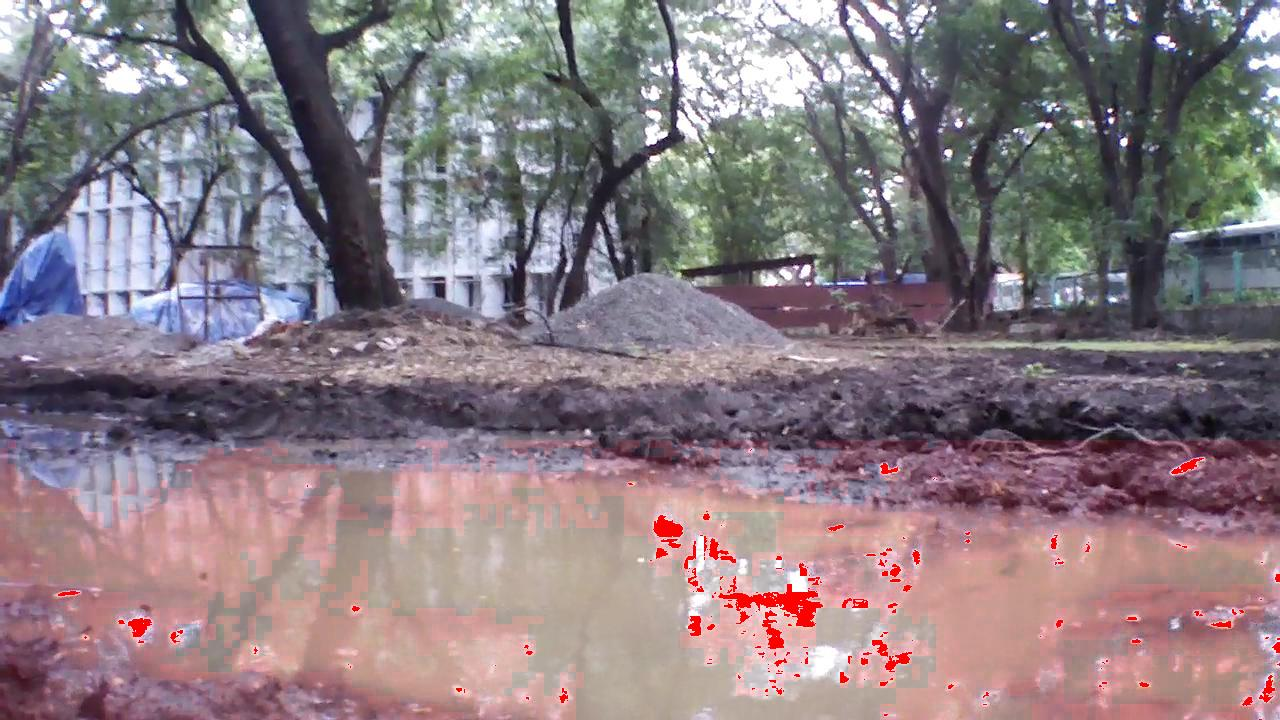
\includegraphics[width=0.31\linewidth]{images/results/dataset_63full/output_102.jpg}\\

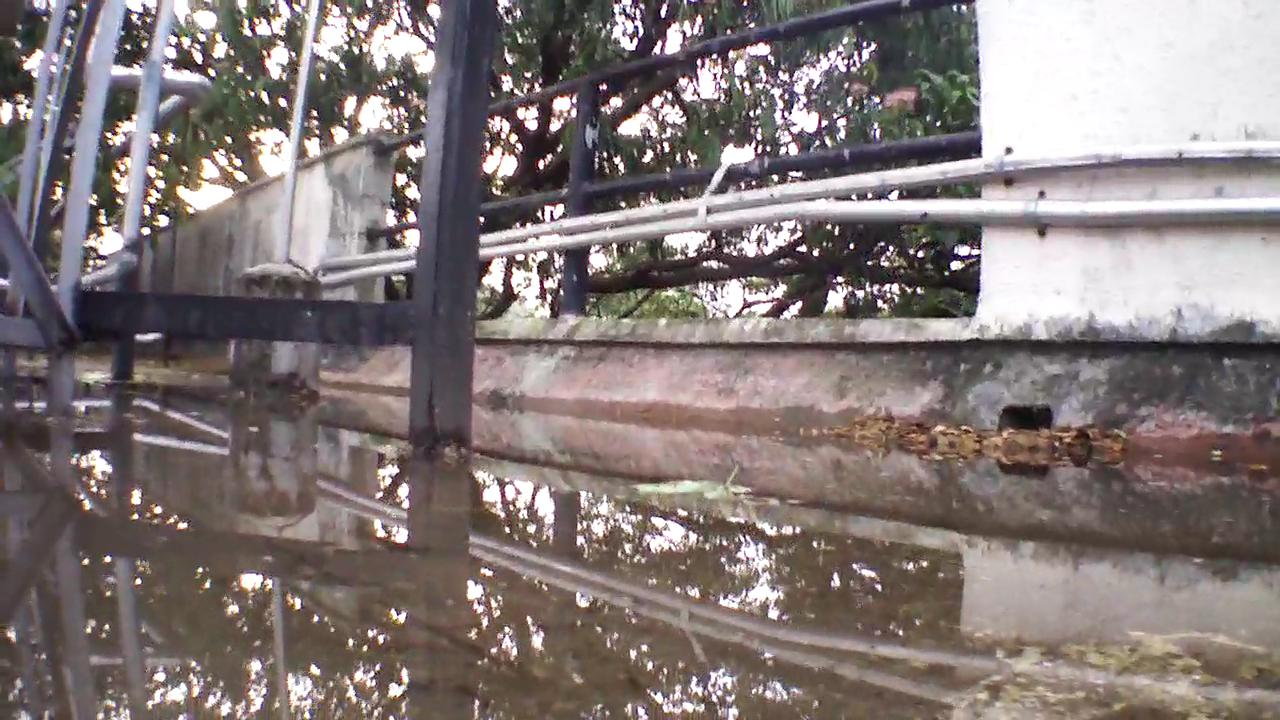
\includegraphics[width=0.31\linewidth]{images/results/dataset_73/IMG_PAIR_124_1.jpg}
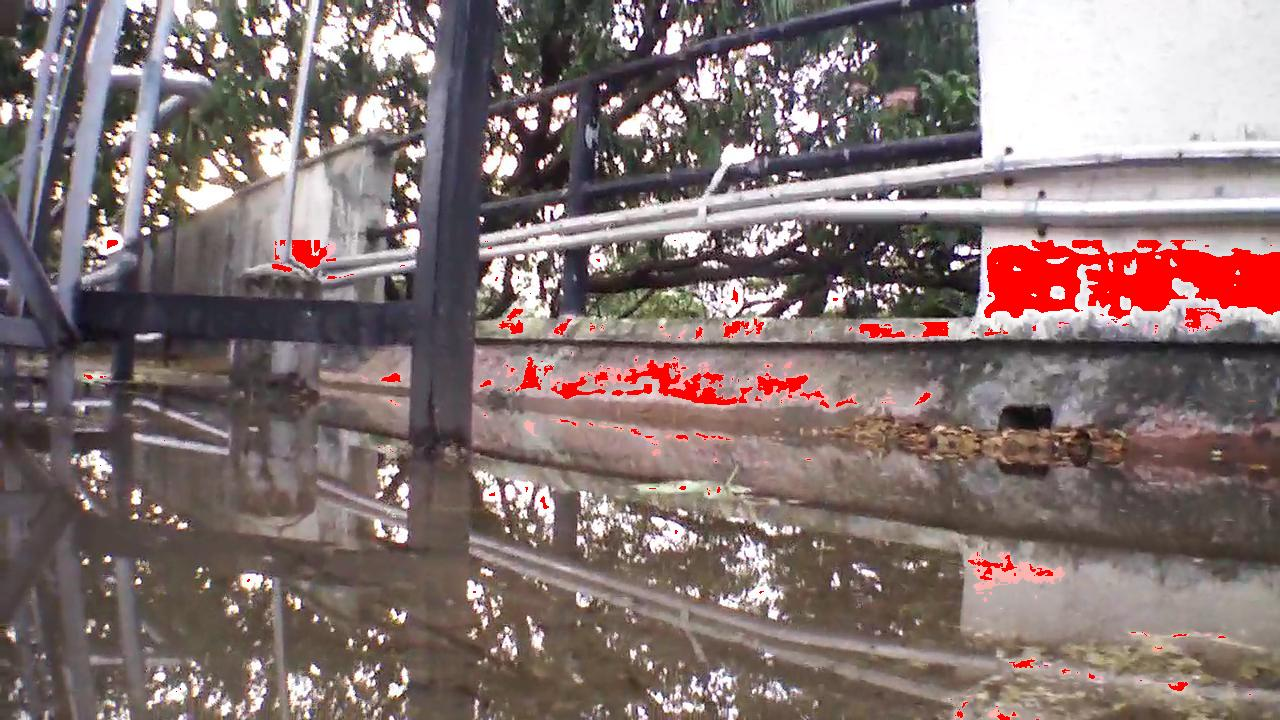
\includegraphics[width=0.31\linewidth]{images/results/dataset_73/output_124_jpl2.jpg}
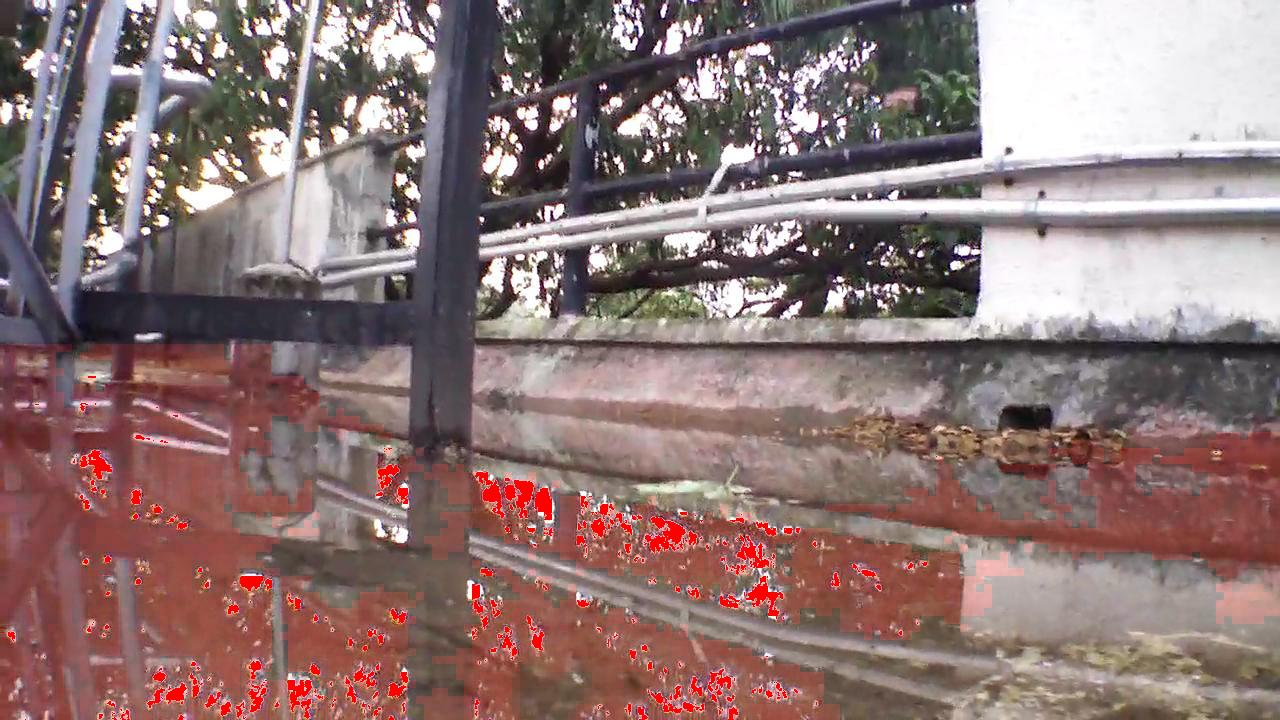
\includegraphics[width=0.31\linewidth]{images/results/dataset_73/output_124.jpg}\\

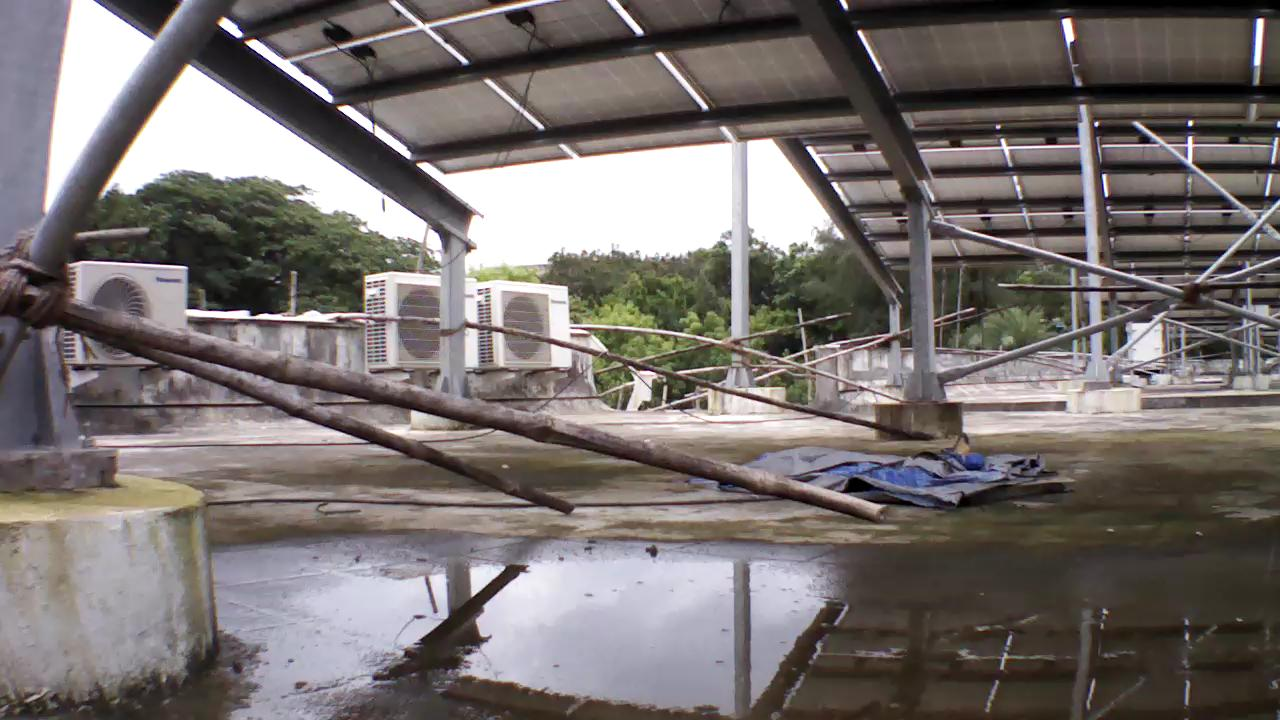
\includegraphics[width=0.31\linewidth]{images/results/dataset_81/IMG_PAIR_1_1.jpg}
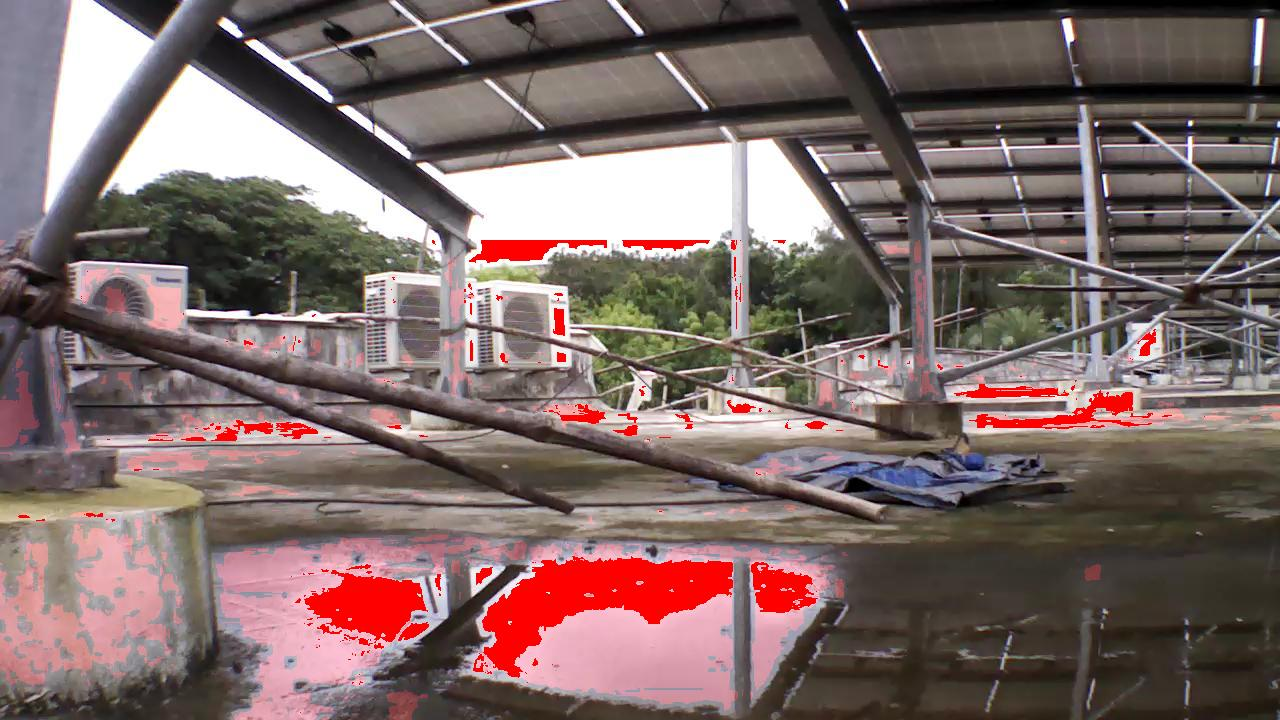
\includegraphics[width=0.31\linewidth]{images/results/dataset_81/output_1_jpl2.jpg}
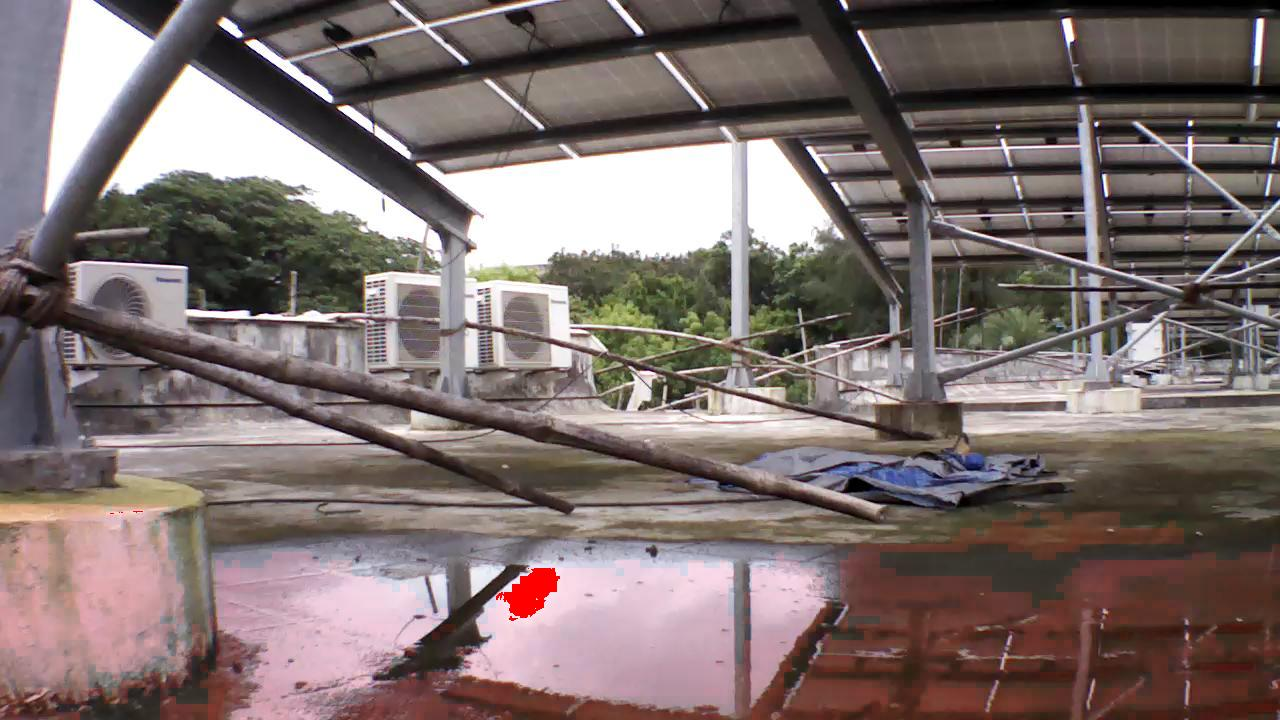
\includegraphics[width=0.31\linewidth]{images/results/dataset_81/output_1.jpg}\\

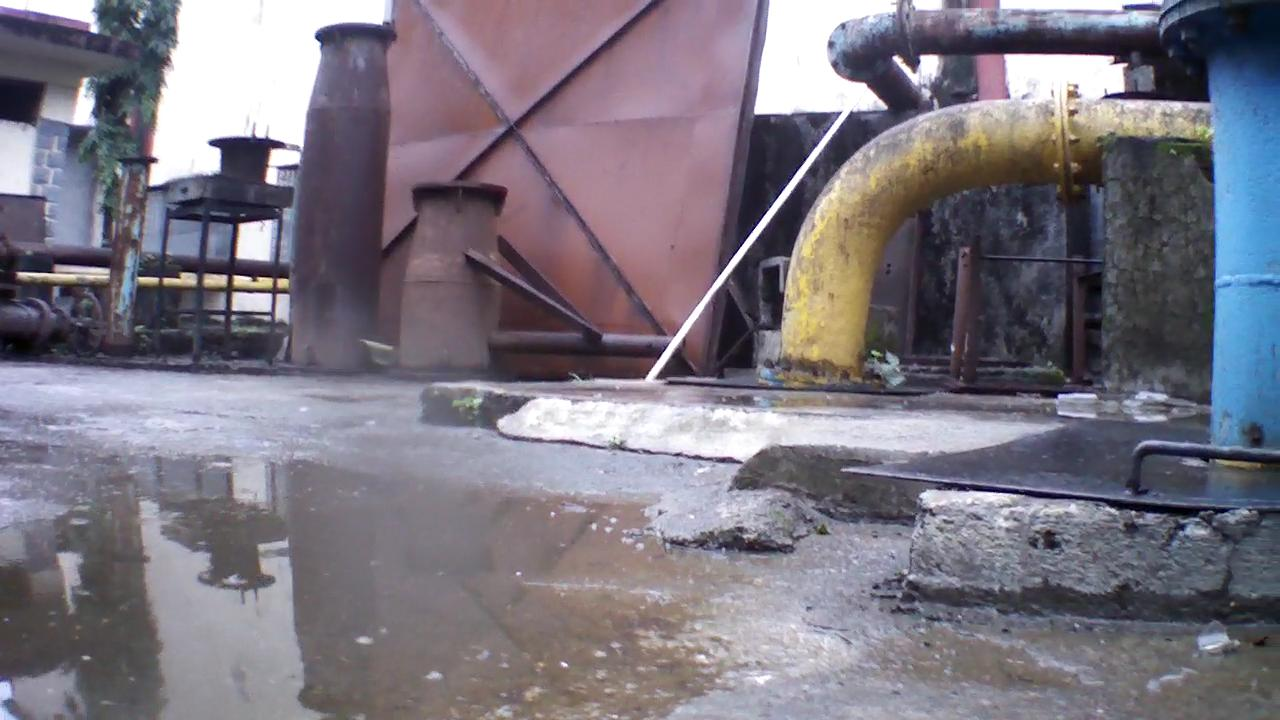
\includegraphics[width=0.31\linewidth]{images/results/dataset_82/IMG_PAIR_192_1.jpg}
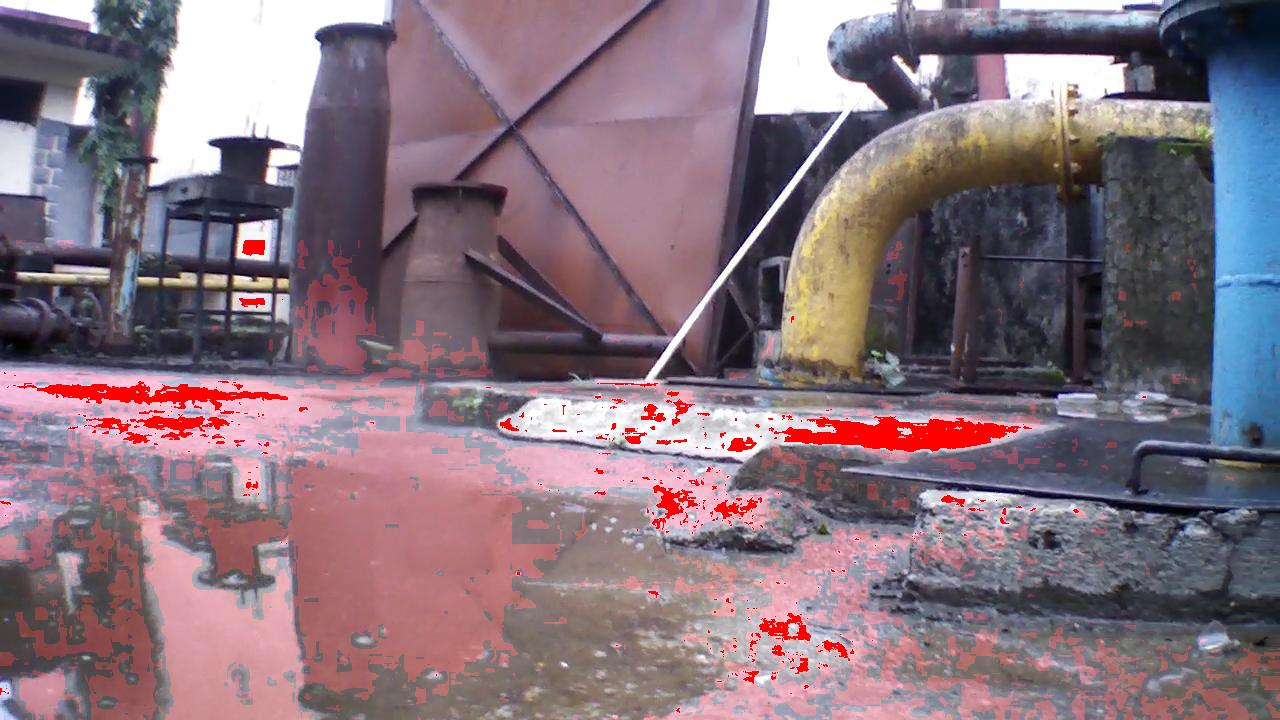
\includegraphics[width=0.31\linewidth]{images/results/dataset_82/output_192_jpl2.jpg}
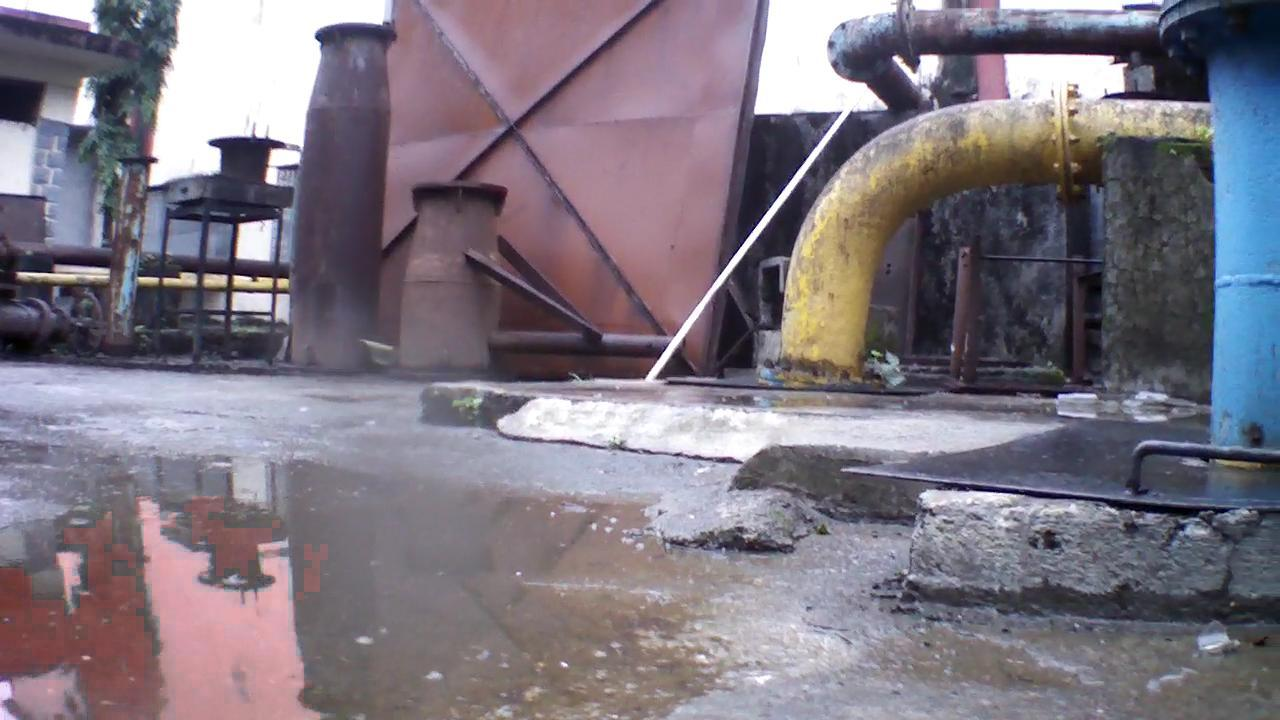
\includegraphics[width=0.31\linewidth]{images/results/dataset_82/output_192.jpg}\\
	
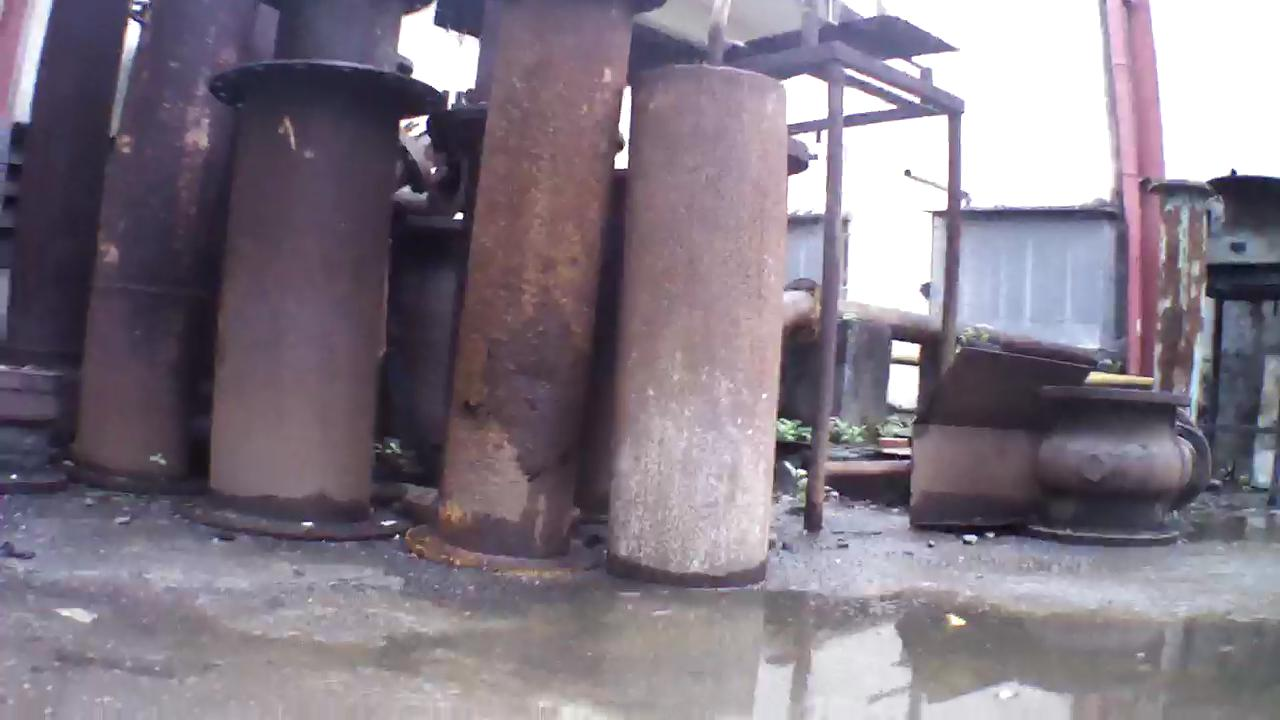
\includegraphics[width=0.31\linewidth]{images/results/dataset_83/IMG_PAIR_130_1.jpg}
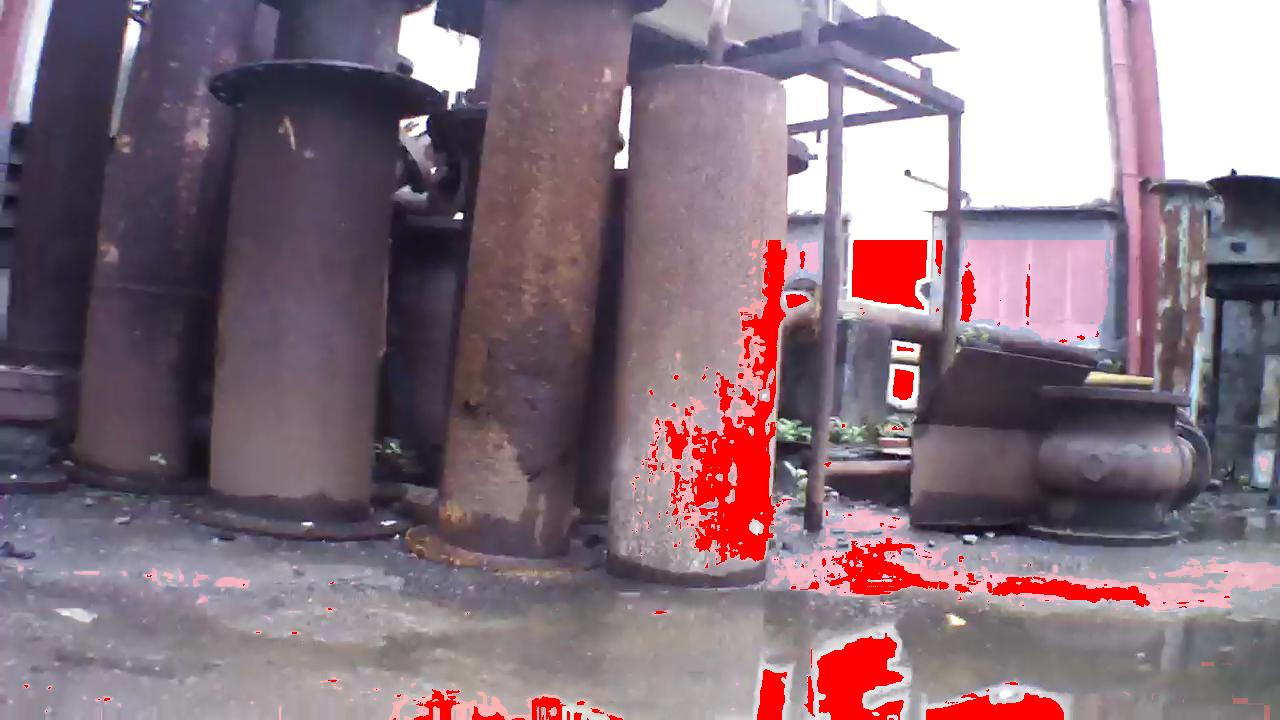
\includegraphics[width=0.31\linewidth]{images/results/dataset_83/output_130_jpl2.jpg}
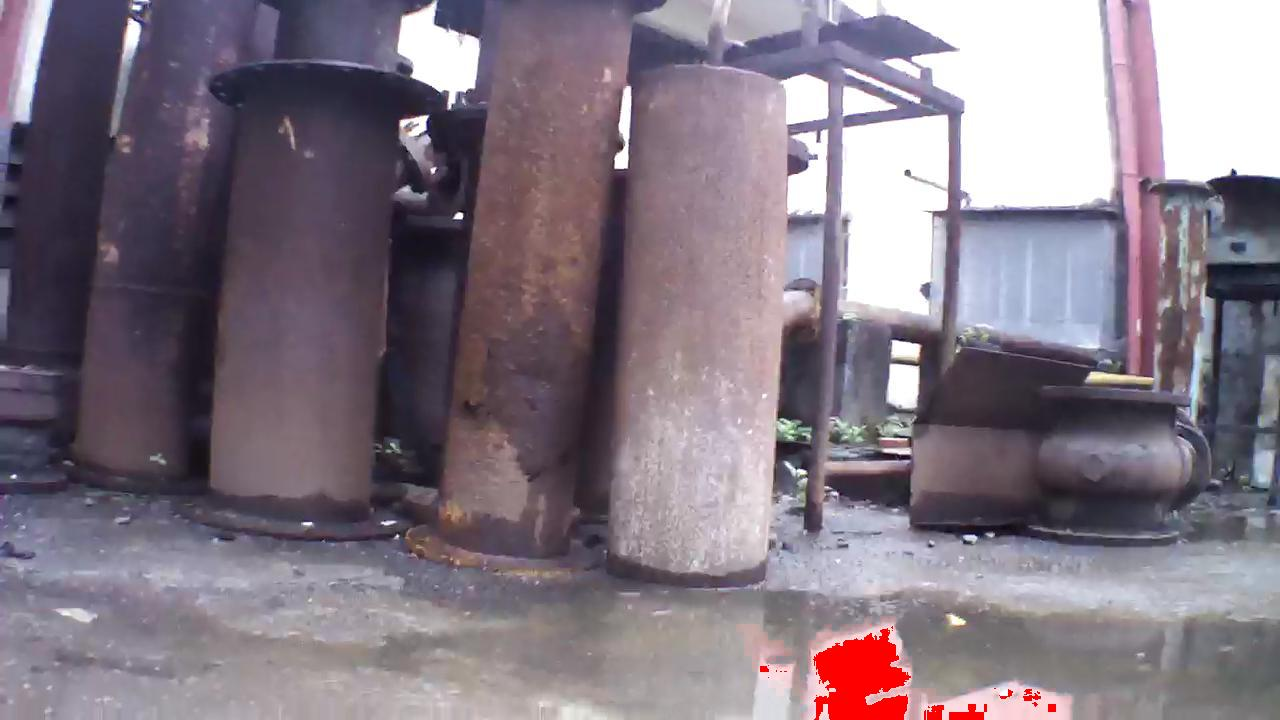
\includegraphics[width=0.31\linewidth]{images/results/dataset_83/output_130.jpg}\\
	
\caption{Comparison of proposed method with Rankin et al.~\cite{rankin04}.
\textbf{Left:} Original Image, \textbf{Middle:} Output of Rankin et
al.~\cite{rankin04}'s method, \textbf{Right:} Proposed method's output. It can
be seen that Rankin et al's method is not able to detect textured puddle
regions. Also, it is getting confused with high intesity non-puddle patches as
puddle patches. While our method is detecting the puddle regions with higher accuracy.}
\label{fig:comparison}
\end{figure}
 
\section{Conclusion and Future Work}
Detection of stagnant water around residential places has become crucial
due to rise in cases of dengue and malaria in urban areas. In this paper, we
proposed a novel technique for detection of inaccessible stagnant-water puddles
in urban areas using aerial devices like quadcopters.
The method proposed involved assigning a probabilistic measure to image patches
in input image frames, indicating likelihood of it being a puddle. The measure
was obtained by combined by scores from a pre-trained SVM-based classifier and
optical flow from suitable consecutive image frames. It is shown that
qualitatively our approach produces better results in a variety of urban
scenarios.

Although the work done in the current paper produces favourable results for
given scenarios. Nevertheless, the results can be improved and the scope
extended in the following directions:
\begin{itemize}
  \item Determination of Horizon from environmental cues could be improved and made
  more robust in order to deal with factors such as illumination changes,
  occlusions and unavailability of artifacts. Also, the parameters involved
  could be automatically estimated through training.
  \item The score obtained from optical flow magnitudes could be improved by
  using the directional components separately, and combine them with
  corresponding quadcopter motion vectors like velocity and acceleration.
  \item The feature using for classifier to obtain the SVM score could be
  modified to produce greater separation between puddle and non-puddle region
  patches.
\end{itemize}

\bibliographystyle{IEEEtran}
\bibliography{egbib}
\end{document}
